\documentclass[../Carre_nights.tex]{subfiles}

\begin{document}

\section{n0000(1)}
\textbf{\Large{The tale of king Shahry\=ar and of his brother, king Shahzam\=an}} \\

\begin{figure}[ht]
\centering
\includegraphics[height=\figsize]{illustrations/volume_1/T01, n0000(1) - Histoire du roi Schahriar et de son frère, le roi Schahzaman.jpg}
\end{figure}

\textit{\\
"...cette colonne se changea en un genni de haute taille, de forte carrure et de large poitrine, et qui portait sur sa tête une caisse. Il mit pied à terre et vint vers l’arbre sur lequel ils étaient et se tint au-dessous. Il enleva alors le couvercle de la caisse et en tira une grande boîte qu’il ouvrit, et aussitôt apparut une jeune fille désirable, éclatante de beauté, lumineuse à l’égal du soleil..."} \\
—T01, n0000(1) - Histoire du roi Schahriar et de son frère, le roi Schahzaman \\~\\
\textit{"...the smoke column changed to a Jinn\={\i} of great size, vast-shouldered, gigantically-breasted, and carrying on his head a box. He put foot to the earth, came towards the tree in which they were, and stopped below it. Then he lifted the lid of the box and took from it a large coffer which he also opened; and thereupon appeared a desirable young girl, bright in her beauty, shining like the sun."} \\
—V01, n0000(1) - The tale of king Shahry\=ar and of his brother, king Shahzam\=an

\newpage

\section{n0000(2)}
\textbf{\Large{The tale of king Shahry\=ar and of his brother, king Shahzam\=an}} \\

\begin{figure}[ht]
\centering
\includegraphics[height=\figsize]{illustrations/volume_1/T01, n0000(2) - Histoire du roi Schahriar et de son frère, le roi Schahzaman.jpg}
\end{figure}

\textit{\\
"...le Roi envoya chercher la petite sœur qui vint et se jeta au cou de Schahrazade, et finit par se blottir auprès du lit. Alors le Roi se leva, et, prenant la vierge Schahrazade, il lui ravit sa virginité. Puis on se mit à causer."} \\
—T01, n0000(2) - Histoire du roi Schahriar et de son frère, le roi Schahzaman \\~\\
\textit{"...the King sent for the little sister, who came and threw herself upon the neck of Shahraz\=ad, and lastly cowered down beside the bed. Then the King rose and, taking the maiden Shahraz\=d, ravished her virginity. Afterwards they spoke together…"} \\
—V01, n0000(2) - The tale of king Shahry\=ar and of his brother, king Shahzam\=an

\newpage

\section{n0003}
\textbf{\Large{The fisherman and jinn\={\i}}} \\

\begin{figure}[ht]
\centering
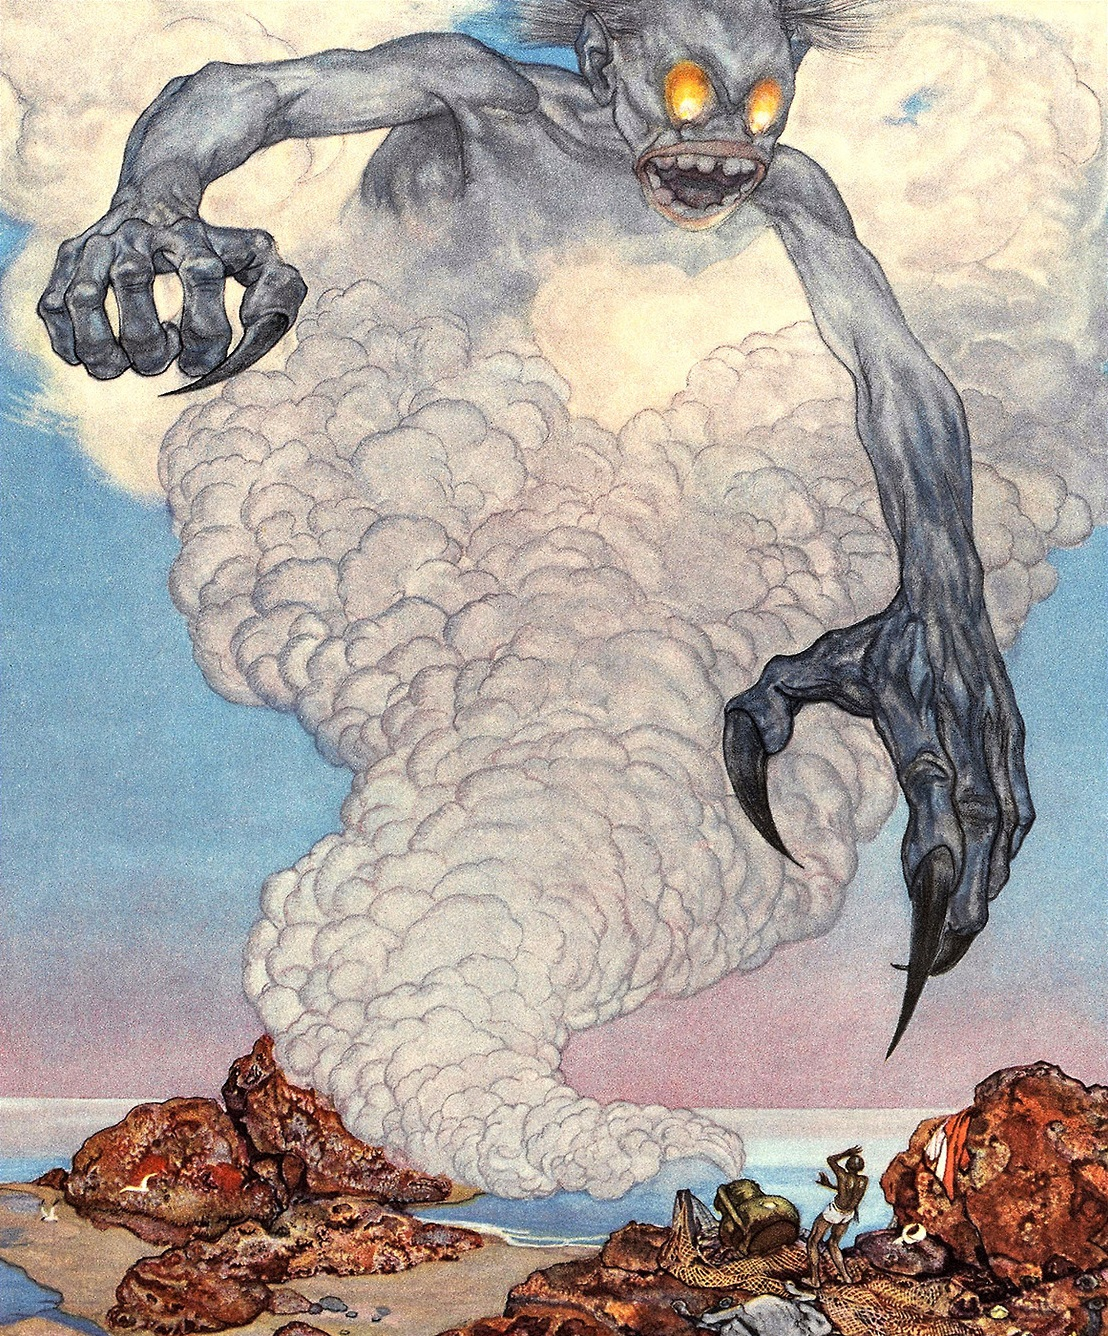
\includegraphics[height=\figsize]{illustrations/volume_1/T01, n0003 - Histoire du pécheur avec l’éfrit.jpg}
\end{figure}

\textit{\\
"...la fumée sortit entièrement, se condensa, se secoua et devint un éfrit dont la tête touchait aux nuages..."} \\
—T01, n0003 - Histoire du pécheur avec l’éfrit \\~\\
\textit{"...the smoke, to the utter amazement of the fisherman, came clear of the vase and, shaking and thickening, turned to an Ifr\={\i}t whose top reached to the clouds…"} \\
—V01, n0003 - The fisherman and jinn\={\i}

\newpage

\section{n0007}
\textbf{\Large{The fisherman and jinn\={\i}}} \\

\begin{figure}[ht]
\centering
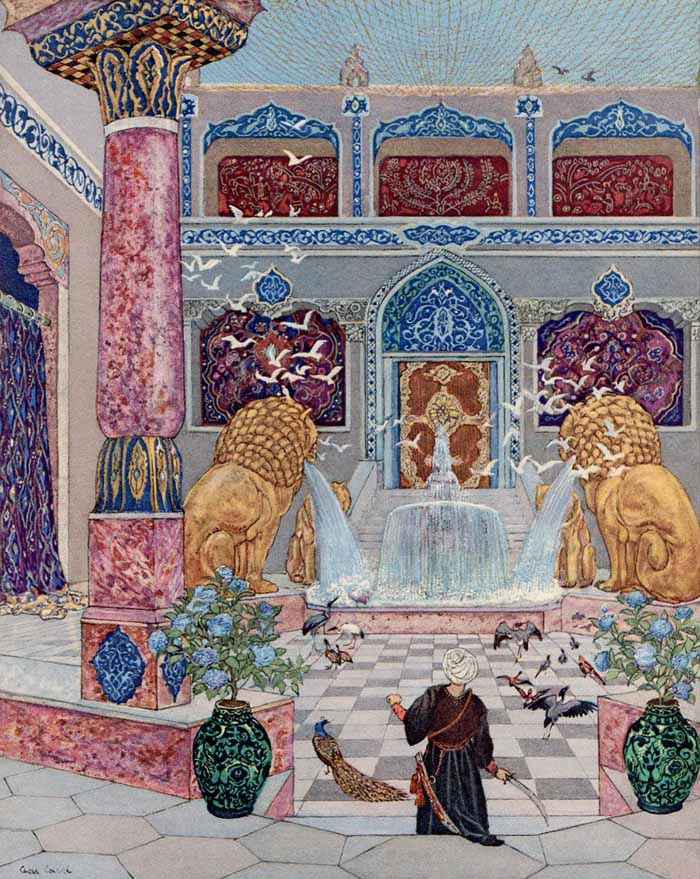
\includegraphics[height=\figsize]{illustrations/volume_1/T01, n0007 - Histoire du pêcheur avec l'éfrit.jpg}
\end{figure}

\textit{\\
"...il vit que tout le palais était somptueusement tendu de tapisseries, et qu’au milieu de la cour intérieure il y avait un bassin surmonté de quatre lions en or rouge et qui laissaient l’eau jaillir de leur gueule en perles éclatantes et en pierreries ; tout autour il y avait de nombreux oiseaux qui ne pouvaient s’envoler hors du palais, empêchés par un large filet qui s’étendait au-dessus du palais."} \\
—T01, n0007 - Histoire du pêcheur avec l'éfrit \\~\\
\textit{"...all the place was splendid with star-wrought tapestries and, in the middle of the inner court, four lions of red gold held up a fountain, spraying so fair a water that it had the appearance of diamonds and white pearls. About the court were many birds, which could not fly away because of a great golden net stretched above the palace."} \\
—V01, n0007 - The fisherman and jinn\={\i}

\newpage

\section{n0009}
\textbf{\Large{The tale of the porter and the young girls}} \\

\begin{figure}[ht]
\centering
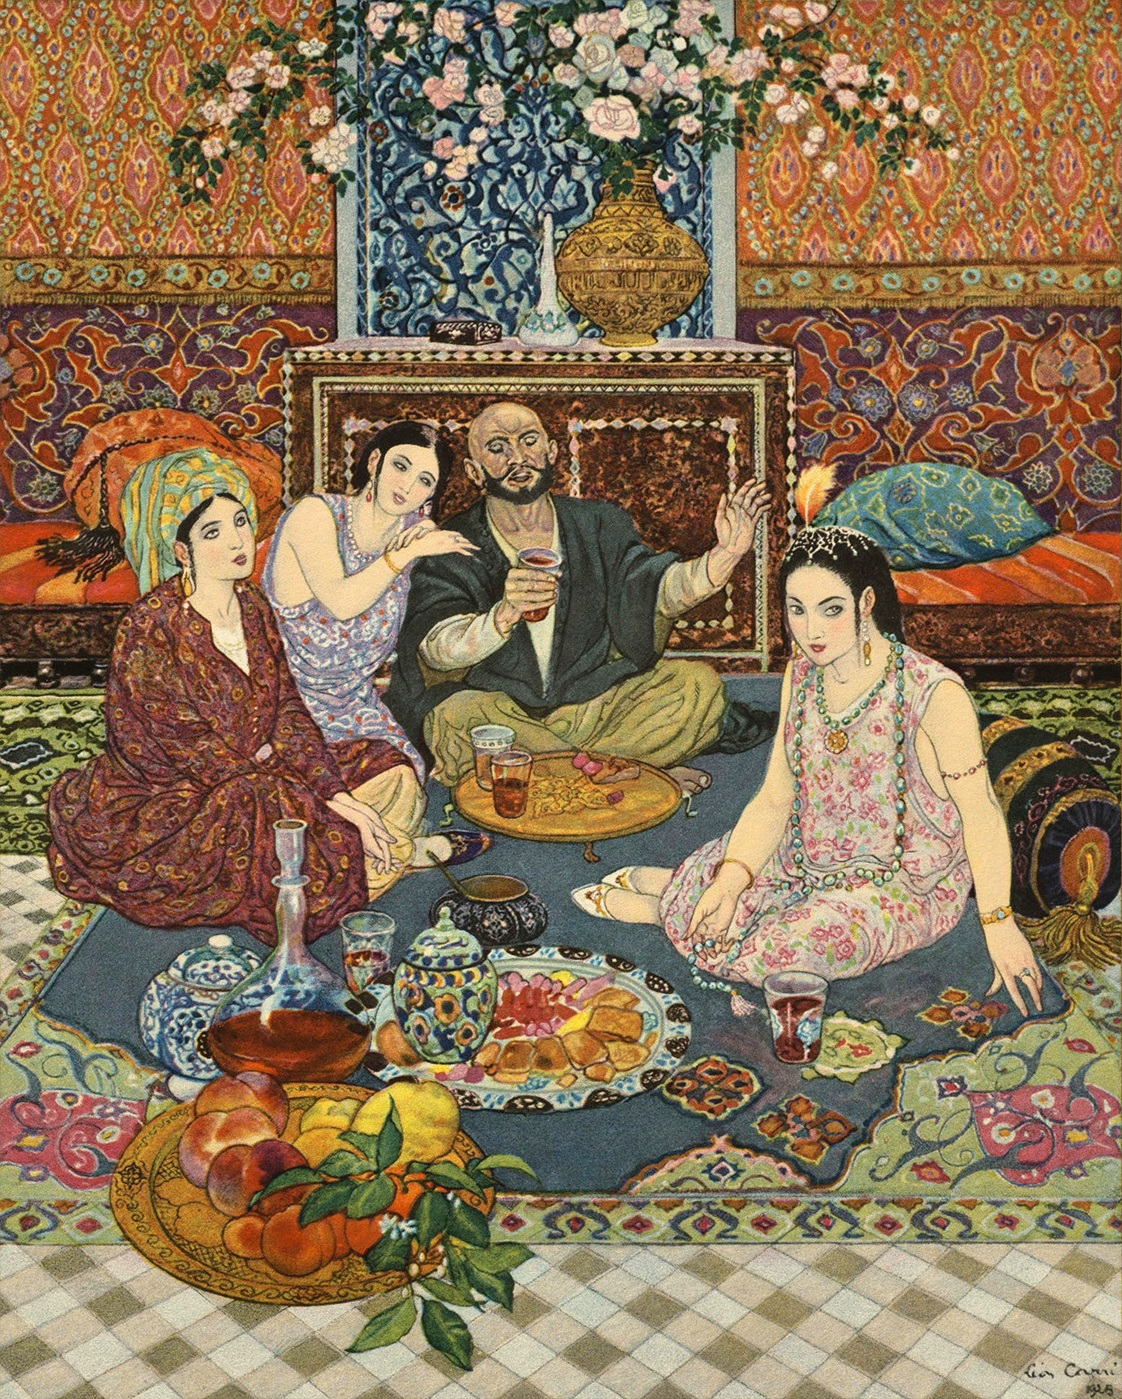
\includegraphics[height=\figsize]{illustrations/volume_1/T01, n0009 - Histoire du portefaix avec les jeunes filles.jpg}
\end{figure}

\textit{\\
"...elle offrit le vin, et tout le monde s’assit ; et le portefaix, au milieu d’elles, s’imaginait qu’il rêvait dans le sommeil."} \\
—T01, n0009 - Histoire du portefaix avec les jeunes filles \\~\\
\textit{"She brought in everything of which they might have need, handed the wine, and saw that all were seated. The porter with these girls on every hand thought that he was dreaming in his sleep."} \\
—V01, n0009 - The tale of the porter and the young girls

\newpage

\section{n0012}
\textbf{\Large{The tale of the porter and the young girls [Tale of the second Kalandar]}} \\

\begin{figure}[ht]
\centering
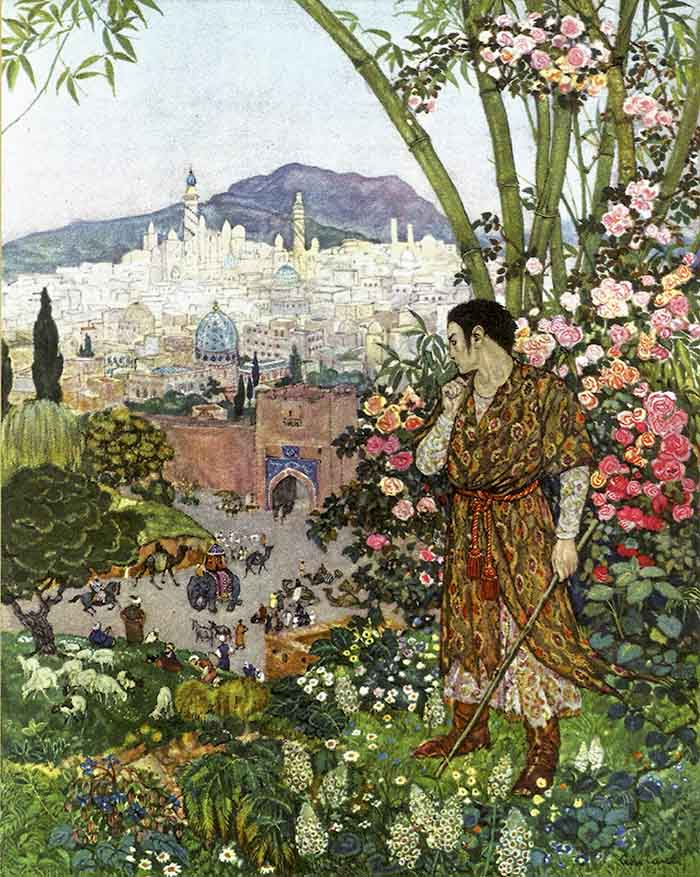
\includegraphics[height=\figsize]{illustrations/volume_1/T01, n0012 - Histoire du portefaix avec les jeunes filles [Histoire du deuxième Saâlouk].jpg}
\end{figure}

\textit{\\
"Le matin, je sortis de la grotte, et je continuai à marcher jusqu’à ce que je fusse arrivé à une ville splendide et prospère, au climat si merveilleux que l’hiver n’avait sur elle aucune prise et que le printemps la couvrait toujours de ses roses."} \\
—T01, n0012 - Histoire du portefaix avec les jeunes filles [Histoire du deuxième Saâlouk] \\~\\
\textit{"Next morning I left the cave and journeyed on until I came to a great and beautiful city, whose air was of such potent balm that Winter might not lay hand upon her but the Spring covered her with his roses all the year."} \\
—V01, n0012 - The tale of the porter and the young girls [Tale of the second Kalandar]

\newpage

\section{n0014}
\textbf{\Large{The tale of the porter and the young girls [Tale of the third Kalandar]}} \\

\begin{figure}[ht]
\centering
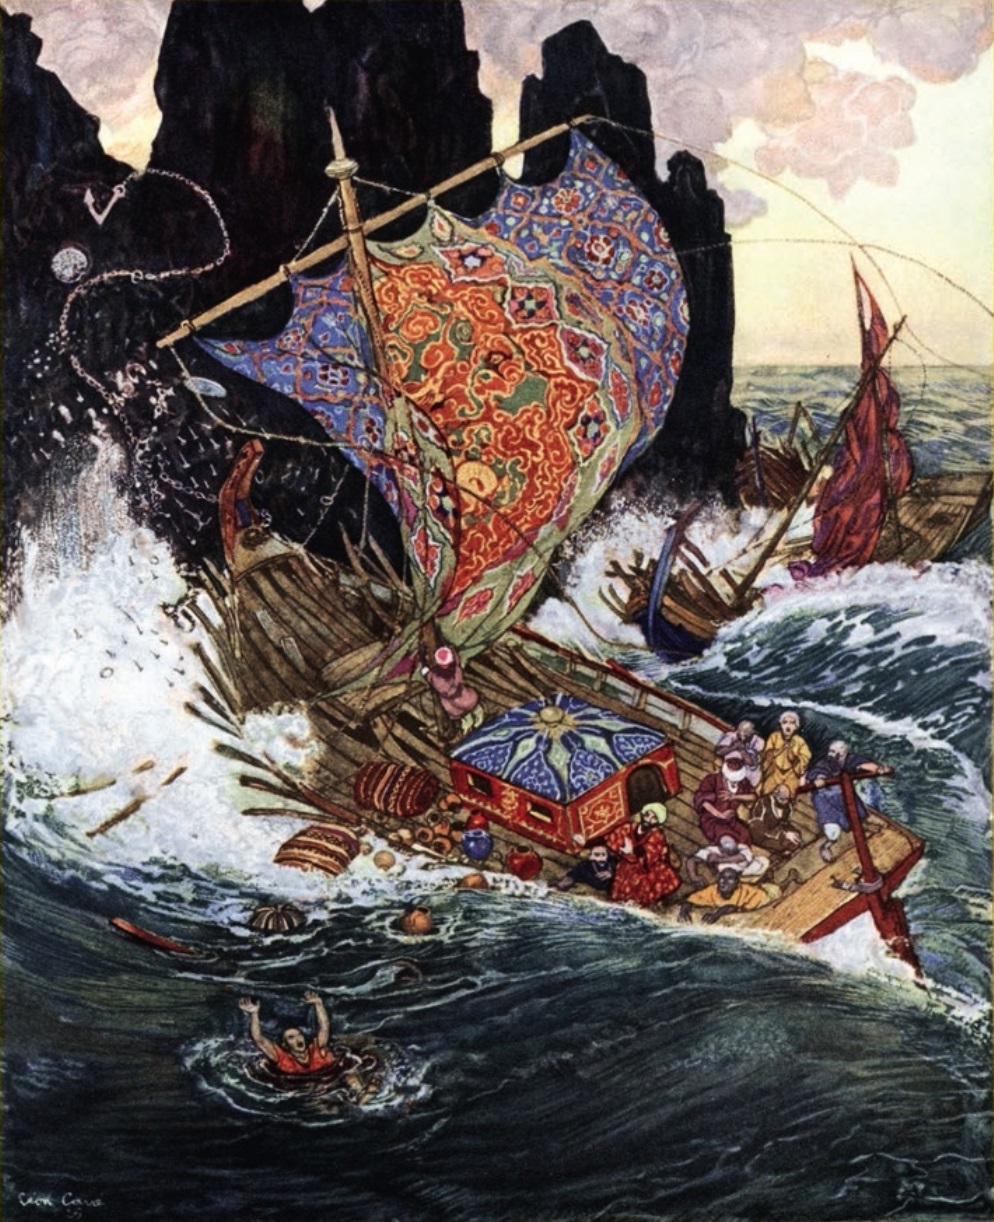
\includegraphics[height=\figsize]{illustrations/volume_1/T01, n0014 - Histoire du portefaix avec les jeunes filles [Histoire du troisième Saâlouk].jpg}
\end{figure}

\textit{\\
"...tout d’un coup les clous des navires se mirent à s’envoler par milliers, avec tous les fers, et allèrent se coller sur la montagne ; et nos navires s’entr’ouvrirent et nous fûmes tous précipités à la mer."} \\
—T01, n0014 - Histoire du portefaix avec les jeunes filles [Histoire du troisième Saâlouk] \\~\\
\textit{"...all the thousands of nails on our ten ships were suddenly wrenched away and flew to join themselves to the mountain. The ships opened out and fell asunder, and we were thrown into the sea."} \\
—V01, n0014 - The tale of the porter and the young girls [Tale of the third Kalandar]

\newpage

\section{n0015}
\textbf{\Large{The tale of the porter and the young girls [Tale of the third Kalandar]}} \\

\begin{figure}[ht]
\centering
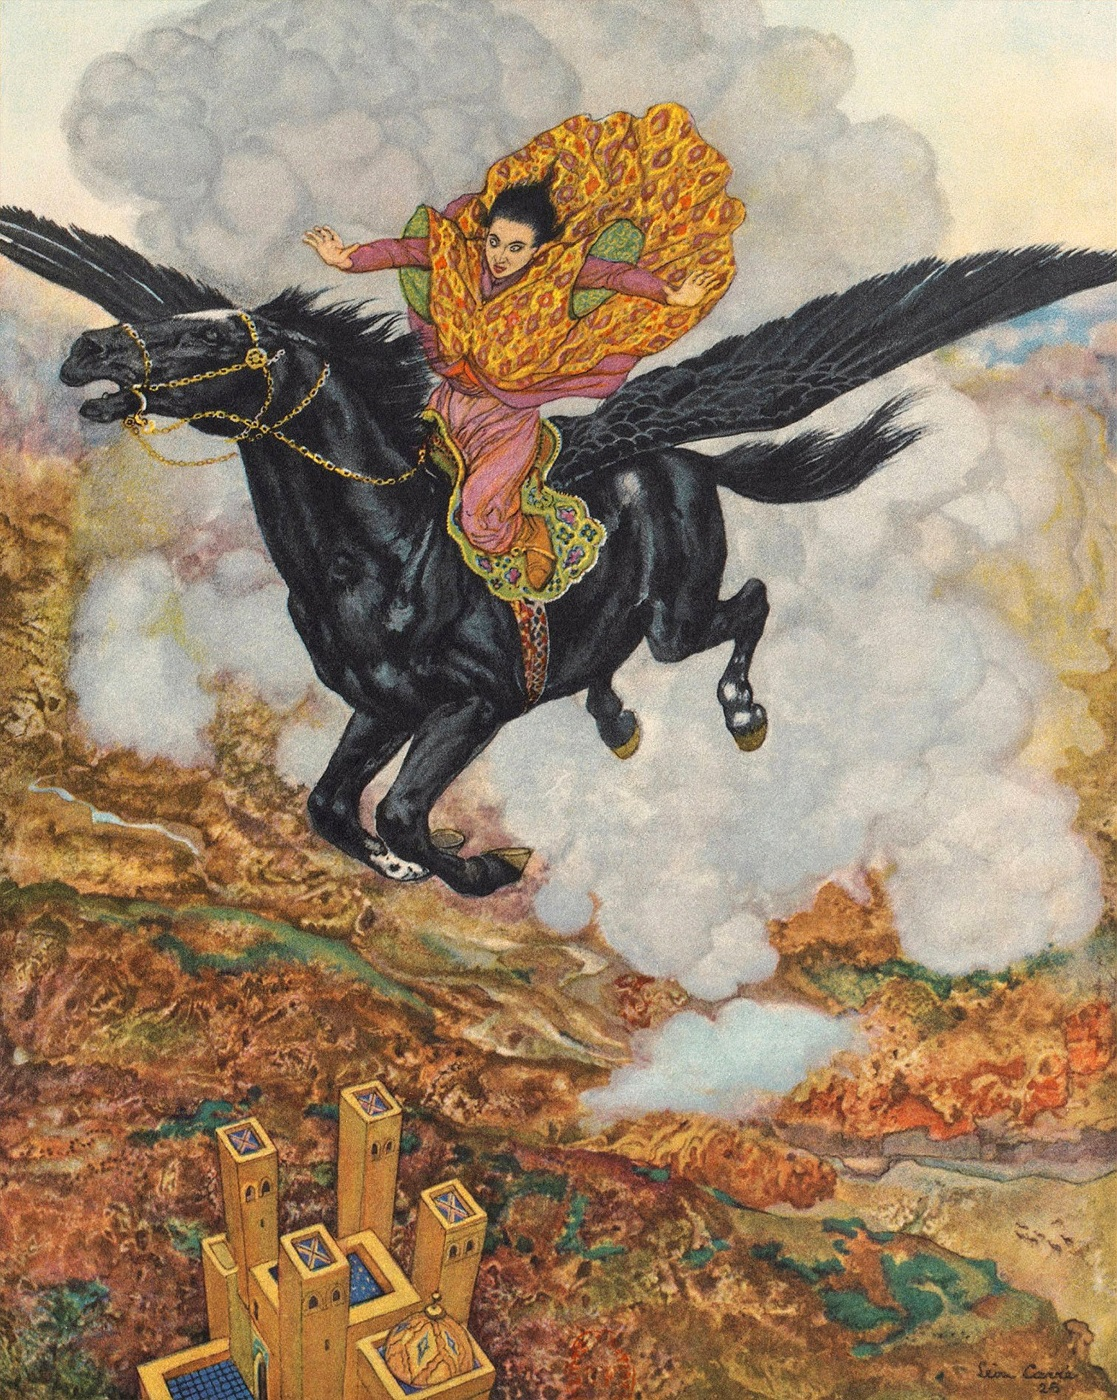
\includegraphics[height=\figsize]{illustrations/volume_1/T01, n0015 - Histoire du portefaix avec les jeunes filles [Histoire du troisième Saâlouk].jpg}
\end{figure}

\textit{\\
"...je le frappai au cou avec la chaîne d’or. Et aussitôt, ô ma maîtresse, le cheval étendit deux grandes ailes noires que je n’avais pas vues jusqu’à cet instant, cria d’une façon épouvantable, frappa trois fois le sol avec son sabot et s’envola avec moi dans les airs."} \\
—T01, n0015 - Histoire du portefaix avec les jeunes filles [Histoire du troisième Saâlouk] \\~\\
\textit{"I slashed him over the neck with the gold chain and at once he spread two mighty black wings which I had not seen, cried out with a terrible voice and, stamping the earth four times with his foot, shot up into the air."} \\
—V01, n0015 - The tale of the porter and the young girls [Tale of the third Kalandar]

\newpage

\section{n0017}
\textbf{\Large{The tale of the porter and the young girls [The tale of the portress Am\={\i}nah]}} \\

\begin{figure}[ht]
\centering
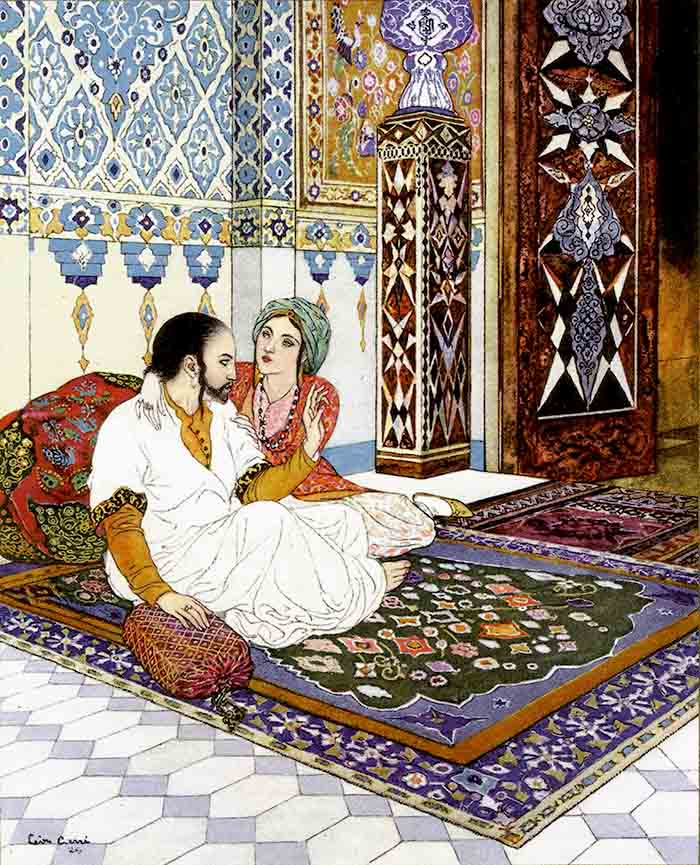
\includegraphics[height=\figsize]{illustrations/volume_1/T01, n0017 - Histoire du portefaix avec les jeunes filles [Histoire d'Amina].jpg}
\end{figure}

\textit{\\
"...il se leva, apporta le Livre Sacré, et me dit : « Tu vas me jurer sur Al-Koran, que jamais tu ne choisiras un autre que moi, et que tu n’auras jamais d’inclination pour un autre ! »"} \\
—T01, n0017 - Histoire du portefaix avec les jeunes filles [Histoire d'Amina] \\~\\
\textit{"He rose and brought the sacred book to me, saying:  I wish you to swear on the Koran never to choose another than I, never to incline towards another. "} \\
—V01, n0017 - The tale of the porter and the young girls [The tale of the portress Am\={\i}nah]

\newpage

\section{n0018(1)}
\textbf{\Large{The tale of the porter and the young girls}} \\

\begin{figure}[ht]
\centering
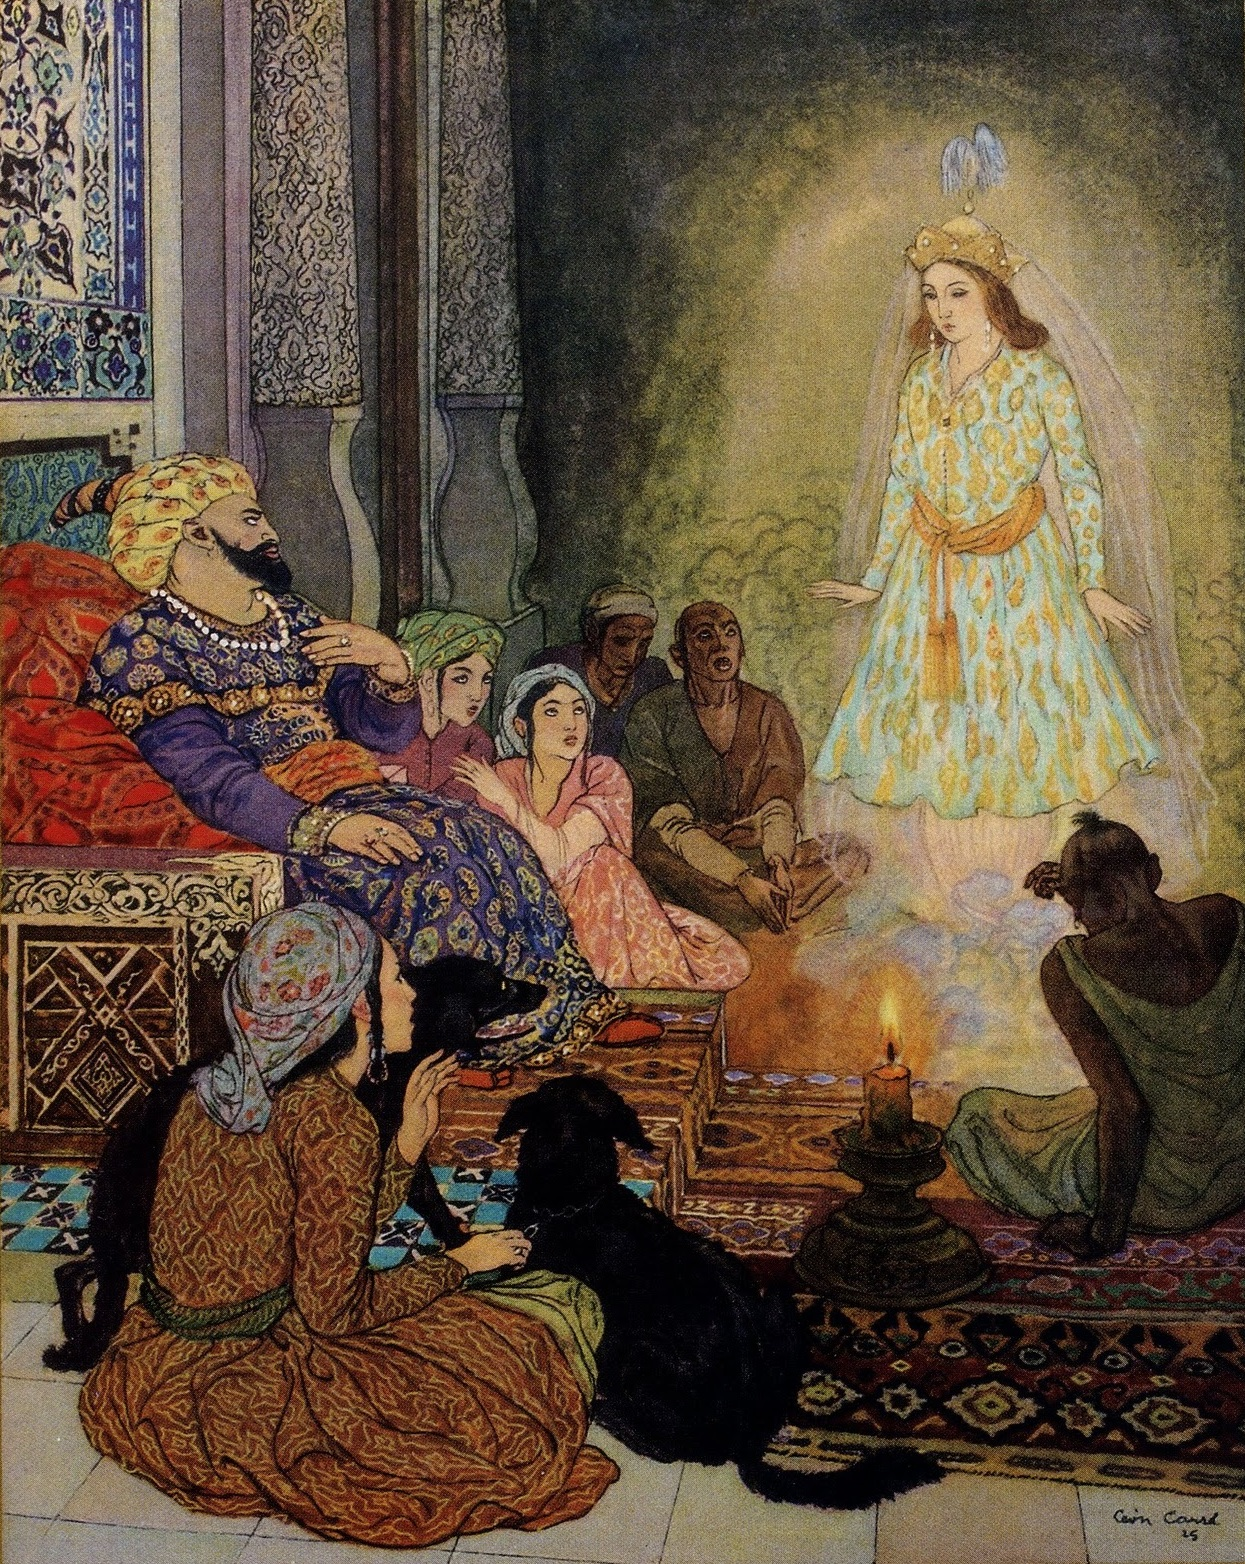
\includegraphics[height=\figsize]{illustrations/volume_1/T01, n0018(1) - Histoire du portefaix avec les jeunes filles.jpg}
\end{figure}

\textit{\\
"...à peine fut sentie l’odeur du cheveu brûlé, qu’il y eut un tremblement dans tout le palais, et une forte secousse ; et tout à coup la gennia apparut sous la forme d’une jeune fille richement habillée."} \\
—T01, n0018(1) - Histoire du portefaix avec les jeunes filles \\~\\
\textit{"No sooner had they smelt the smell of burning hair than the palace shook as at a great blow and the Jinn\={\i}yah stood before them in the likeness of a richly-habited young girl."} \\
—V01, n0018(1) - The tale of the porter and the young girls

\newpage

\section{n0018(2)}
\textbf{\Large{The tale of the woman cut in pieces}} \\

\begin{figure}[ht]
\centering
\includegraphics[height=\figsize]{illustrations/volume_1/T01, n0018(2) - Histoire de la femme coupée.jpg}
\end{figure}

\textit{\\
"...je passai toute la nuit à penser au moyen de trouver une pomme. Le lendemain, à l’aube, je sortis de ma maison et me dirigeai vers les jardins et me mis à les visiter un par un, arbre par arbre…"} \\
—T01, n0018(2) - Histoire de la femme coupée \\~\\
\textit{"I studied all night how I might come by the fruit and at dawn made my way to the market-gardens, visiting them one by one, and tree by tree."} \\
—V01, n0018(2) - The tale of the woman cut in pieces

\newpage

\section{n0020}
\textbf{\Large{The tale of the waz\={\i}r N\=ur Al-d\={\i}}} \\

\begin{figure}[ht]
\centering
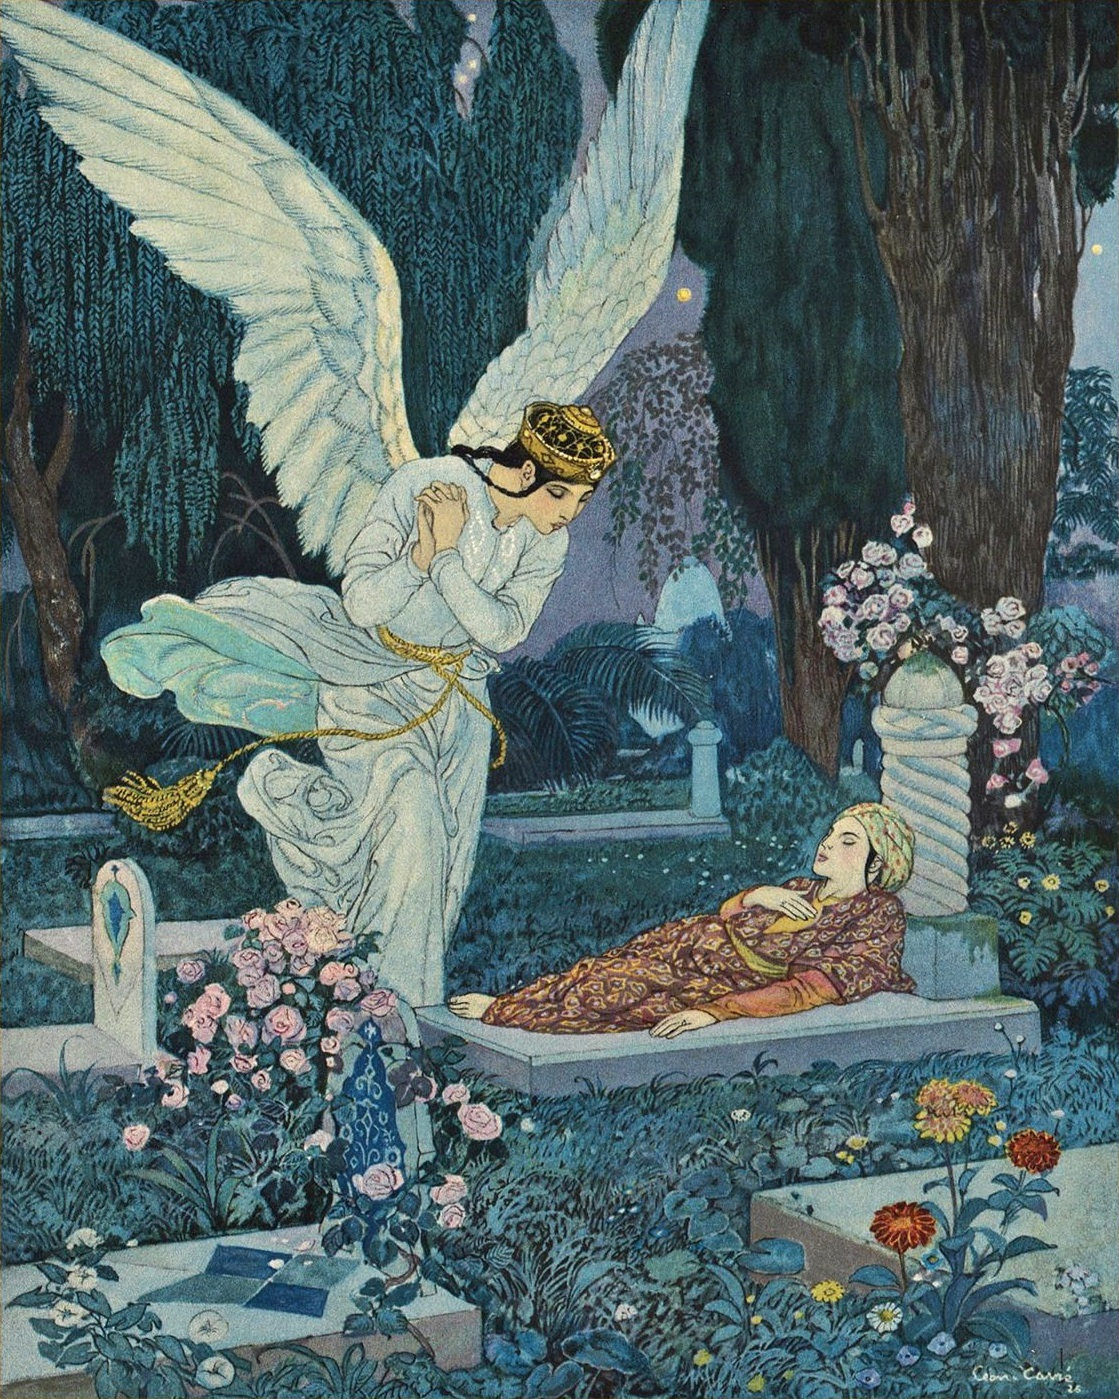
\includegraphics[height=\figsize]{illustrations/volume_1/T01, n0020 - Histoire du vizir Noureddine.jpg}
\end{figure}

\textit{\\
"...une charmante gennia prenait l’air à cette heure, sous les rayons de la lune, et, dans sa promenade, passa à côté de Hassan endormi, et le vit, et remarqua sa beauté et ses belles proportions, et elle fut fort émerveillée..."} \\
—T01, n0020 - Histoire du vizir Noureddine \\~\\
\textit{"...a charming Jinn\={\i}yah was taking the air at that time under the moonlight, and happening to pass by the sleeping Hasan she halted on seeing his surpassing beauty."} \\
—V01, n0020 - The tale of the waz\={\i}r N\=ur Al-d\={\i}

\newpage

\section{n0027(1)}
\textbf{\Large{The tale of the hunchback [The tale of the steward]}} \\

\begin{figure}[ht]
\centering
\includegraphics[height=\figsize]{illustrations/volume_1/T01, n0027(1) - Histoire du bossu [Récit de l'intendant du roi de la Chine].jpg}
\end{figure}

\textit{\\
"...un jour que j’étais assis dans ma boutique, je vis une adolescente, et de ma vie je ne vis de mes yeux quelque chose de plus beau. Elle était habillée de vêtements magnifiques, et était montée sur une mule. Devant elle, marchait un eunuque et, derrière elle, un autre eunuque."} \\
—T01, n0027(1) - Histoire du bossu [Récit de l'intendant du roi de la Chine] \\~\\
\textit{"One day I was sitting in my shop when I beheld a girl, the like of whose beauty these eyes had never seen before. She was dressed with unusual magnificence and rode upon a mule; in front of her walked one black eunuch and behind her another."} \\
—V01, n0027(1) - The tale of the hunchback [The tale of the steward]

\newpage

\section{n0027(2)}
\textbf{\Large{The tale of the hunchback [The tale of Jewish doctor]}} \\

\begin{figure}[ht]
\centering
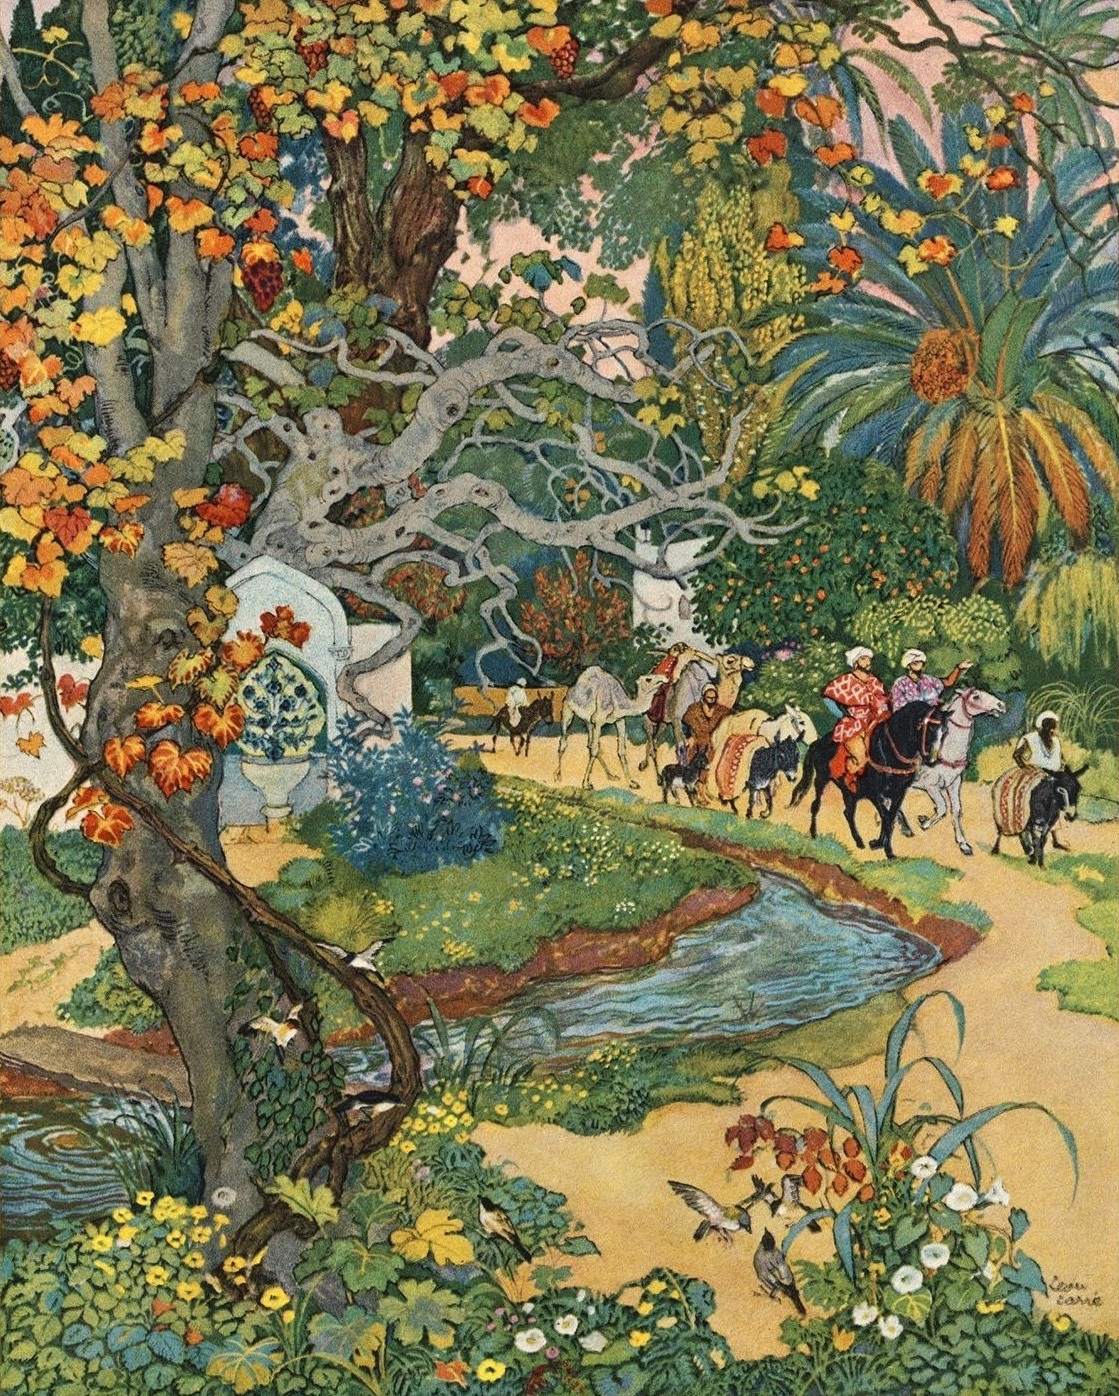
\includegraphics[height=\figsize]{illustrations/volume_1/T01, n0027(2) - Histoire du bossu [Récit du médecin juif].jpg}
\end{figure}

\textit{\\
"...Damas était un lieu enfoui au milieu des jardins, des eaux courantes, des arbres, des fruits et des oiseaux."} \\
—T01, n0027(2) - Histoire du bossu [Récit du médecin juif] \\~\\
\textit{"We found the city of Damascus a place set in the midst of gardens with running waters, trees and birds in excess of all other places."} \\
—V01, n0027(2) - The tale of the hunchback [The tale of Jewish doctor]

\newpage

\section{n0027(3)}
\textbf{\Large{The tale of the hunchback [The tale of Jewish doctor]}} \\

\begin{figure}[ht]
\centering
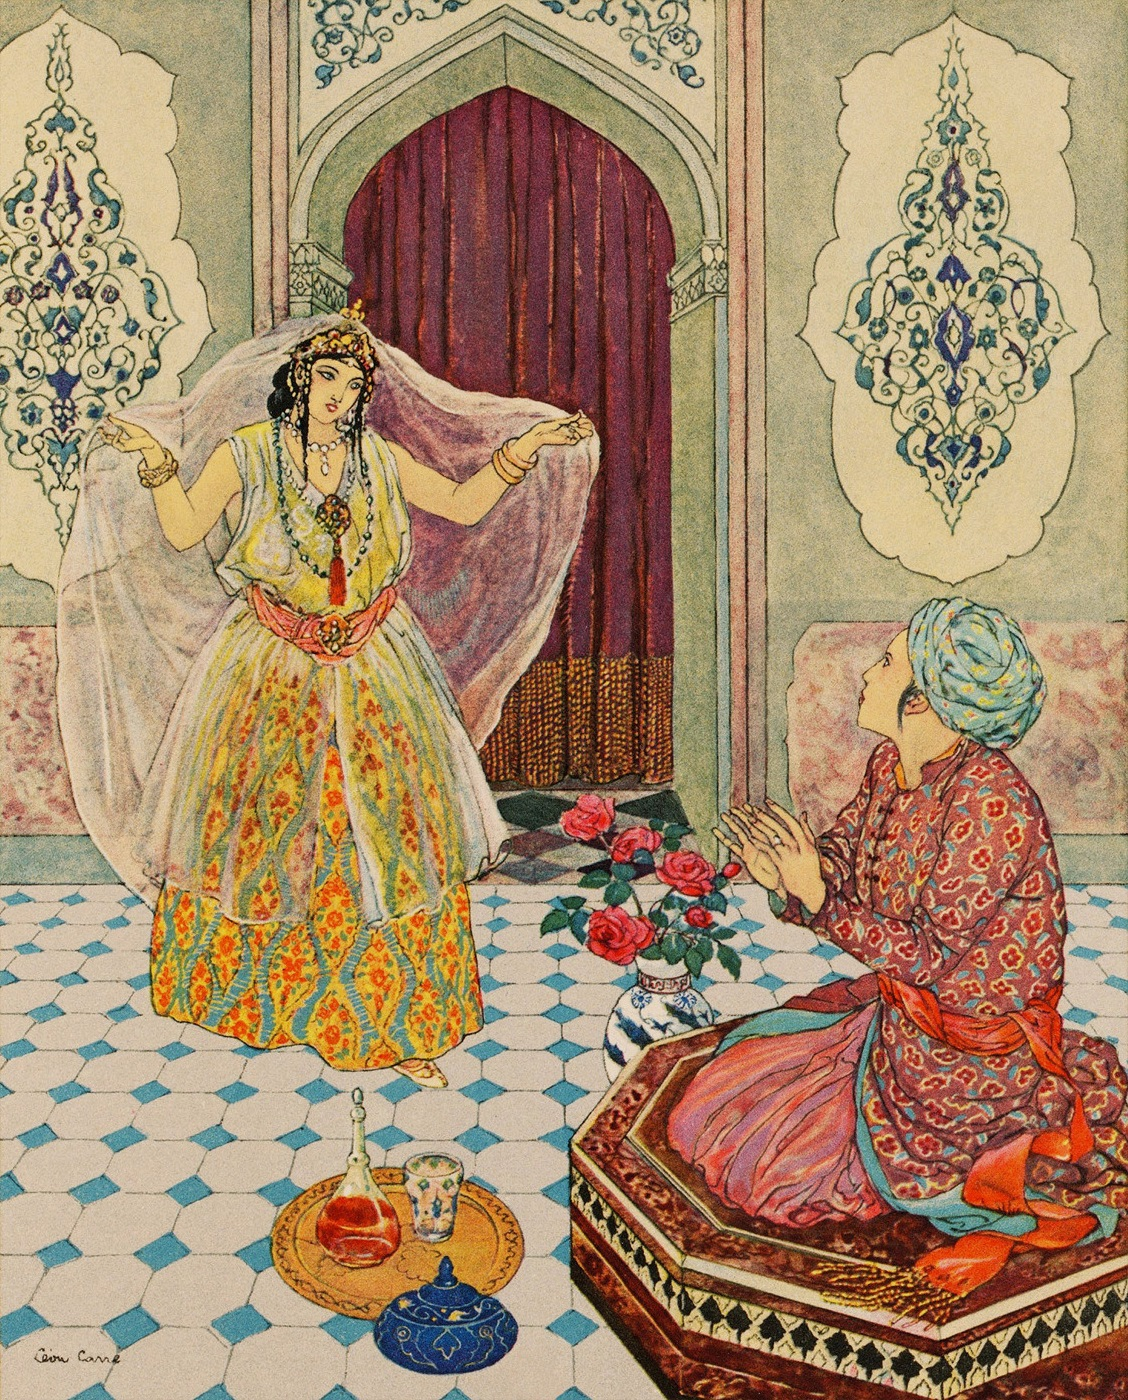
\includegraphics[height=\figsize]{illustrations/volume_1/T01, n0027(3) - Histoire du bossu [Récit du médecin juif].jpg}
\end{figure}

\textit{\\
"...elle se découvrit, enleva son grand voile et m’apparut dans toute sa beauté. Je la trouvai si ravissante que je devins complètement éperdu d’amour."} \\
—T01, n0027(3) - Histoire du bossu [Récit du médecin juif] \\~\\
\textit{"...she took off her veil and appeared in all her beauty, so that I fell into a complete madness of love for her."} \\
—V01, n0027(3) - The tale of the hunchback [The tale of Jewish doctor]

\newpage

\section{n0028}
\textbf{\Large{The tale of the hunchback [The tale of the the lame man]}} \\

\begin{figure}[ht]
\centering
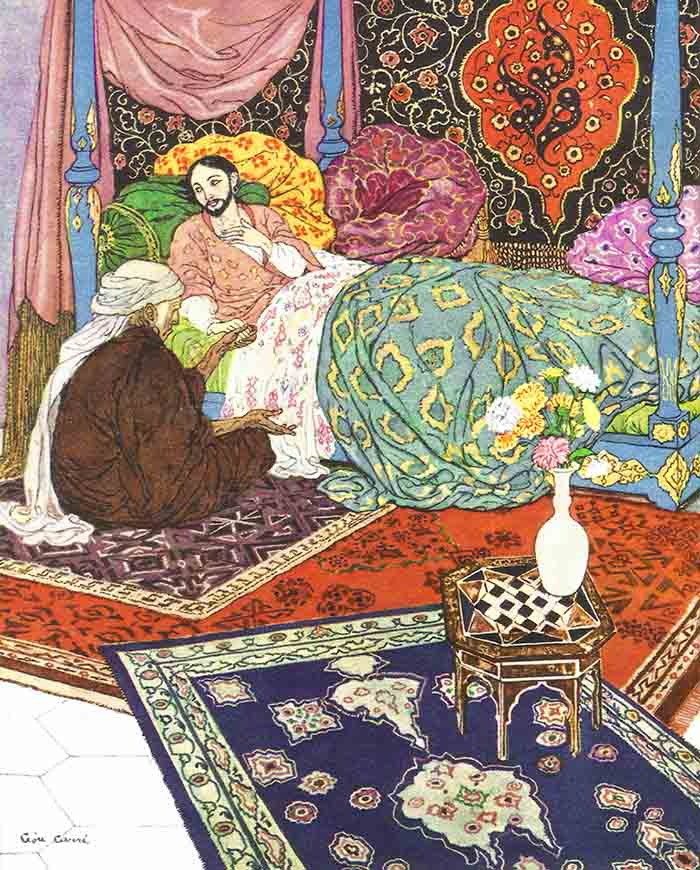
\includegraphics[height=\figsize]{illustrations/volume_1/T01, n0028 - Histoire du bossu [Histoire du jeune homme boiteux].jpg}
\end{figure}

\textit{\\
"Un jour, je vis entrer chez moi une vieille femme qui, au lieu de gémir sur mon état et de me plaindre, vint s’asseoir au chevet de mon lit et se mit à me dire des paroles fort douces pour me calmer…"} \\
—T01, n0028 - Histoire du bossu [Histoire du jeune homme boiteux] \\~\\
\textit{"One day I saw an old woman come into the room who, instead of groaning and weeping over my condition as the others did, sat down and calmed my spirit with sprightly commonplace."} \\
—V01, n0028 - The tale of the hunchback [The tale of the the lame man]

\newpage

\section{n0030}
\textbf{\Large{The tale of the hunchback [The tales of the barber of Baghd\=ad [The tale of Bakb\=uk]]}} \\

\begin{figure}[ht]
\centering
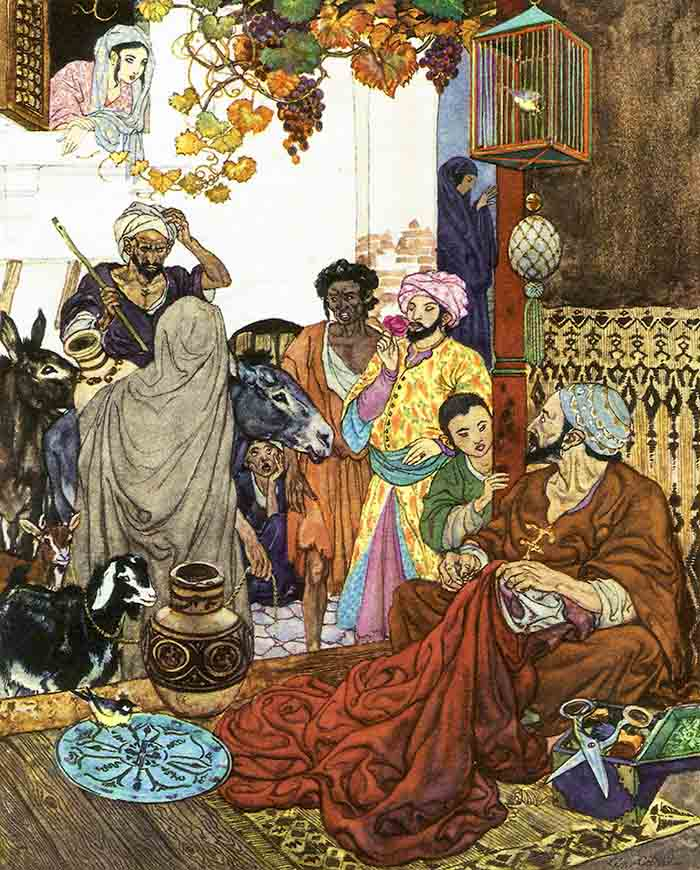
\includegraphics[height=\figsize]{illustrations/volume_1/T01, n0030 - Histoire du bossu [Histoires du barbier de Baghdad [Histoire de Bacbouk]].jpg}
\end{figure}

\textit{\\
"...en levant la tête, il aperçut au-dessus de lui, à la lucarne supérieure, une femme comme la lune à son lever, et qui s’amusait à regarder les passants. C’était l’épouse du propriétaire de la maison. À sa vue, mon frère Bacbouk sentit son cœur s’éprendre passionnément, et il lui fut impossible de coudre ou de faire autre chose que de regarder la lucarne..."} \\
—T01, n0030 - Histoire du bossu [Histoires du barbier de Baghdad [Histoire de Bacbouk]] \\~\\
\textit{"...he chanced to raise his eyes and saw a woman looking out at the passers- by from a skylight let into the terrace floor above him. She was the wife of the owner of the building, and her looking forth was like the rising of the young moon. Bakb\=uk s heart was fired with passion at the sight of her. He could sew no more, but spent all day with his head fixed, looking up at the skylight"} \\
—V01, n0030 - The tale of the hunchback [The tales of the barber of Baghd\=ad [The tale of Bakb\=uk]]

\newpage

\section{n0032(1)}
\textbf{\Large{The tale of the hunchback [The tales of the barber of Baghd\=ad [The tale of al-Ash\=ar]]}} \\

\begin{figure}[ht]
\centering
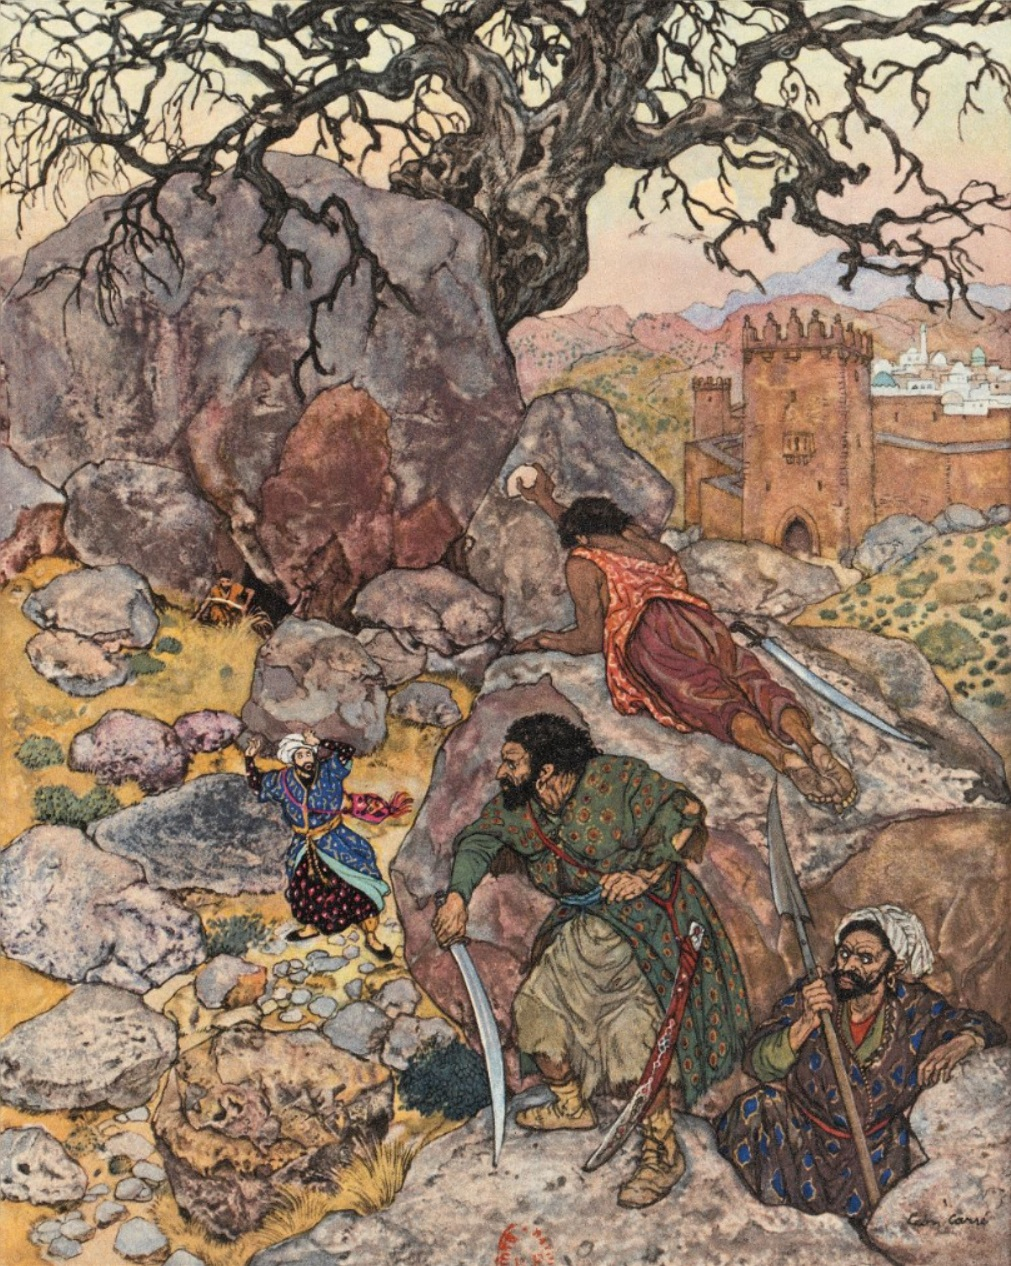
\includegraphics[height=\figsize]{illustrations/volume_1/T01, n0032(1) - Histoire du bossu [Histoires du barbier de Baghdad [Histoire d’El-Aschâr]].jpg}
\end{figure}

\textit{\\
"...mon frère fut ainsi obligé de fuir au loin. Mais, pour que la destinée s’accomplît entièrement, à peine était-il hors des portes de la ville, qu’il fut assailli par des brigands..."} \\
—T01, n0032(1) - Histoire du bossu [Histoires du barbier de Baghdad [Histoire d’El-Aschâr]] \\~\\
\textit{"...he was obliged to leave the city on the instant. That his destiny might be fulfilled he had hardly got beyond the gates when he was set upon by brigands…"} \\
—V01, n0032(1) - The tale of the hunchback [The tales of the barber of Baghd\=ad [The tale of al-Ash\=ar]]

\newpage

\section{n0032(2)}
\textbf{\Large{The tale of the hunchback [The tales of the barber of Baghd\=ad [The tale of Shakk\=ashik]]}} \\

\begin{figure}[ht]
\centering
\includegraphics[height=\figsize]{illustrations/volume_1/T01, n0032(2) - Histoire du bossu [Histoires du barbier de Baghdad [Histoire de Schakâlik]].jpg}
\end{figure}

\textit{\\
"...dès leur entrée, ils furent reçus au son des instruments d’harmonie et aux chants des esclaves blanches toutes plus belles que des lunes. Ces jeunes chanteuses, pendant que mon frère et le vieillard buvaient délicieusement les vins les plus exquis, ne cessèrent de chanter sur tous les tons toutes les mélodies les plus charmantes et avec des modulations et une valeur des sons et un accent admirables."} \\
—T01, n0032(2) - Histoire du bossu [Histoires du barbier de Baghdad [Histoire de Schakâlik]] \\~\\
\textit{"On going in, they were received with lute-playing and singing by white slaves as fair as a flock of summer moons. They sang while my brother and the old man drank the oldest wines, and charmed them with the most pleasing melodies."} \\
—V01, n0032(2) - The tale of the hunchback [The tales of the barber of Baghd\=ad [The tale of Shakk\=ashik]]

\newpage

\section{n0032(3)}
\textbf{\Large{The tale of Sweet-Friend}} \\

\begin{figure}[ht]
\centering
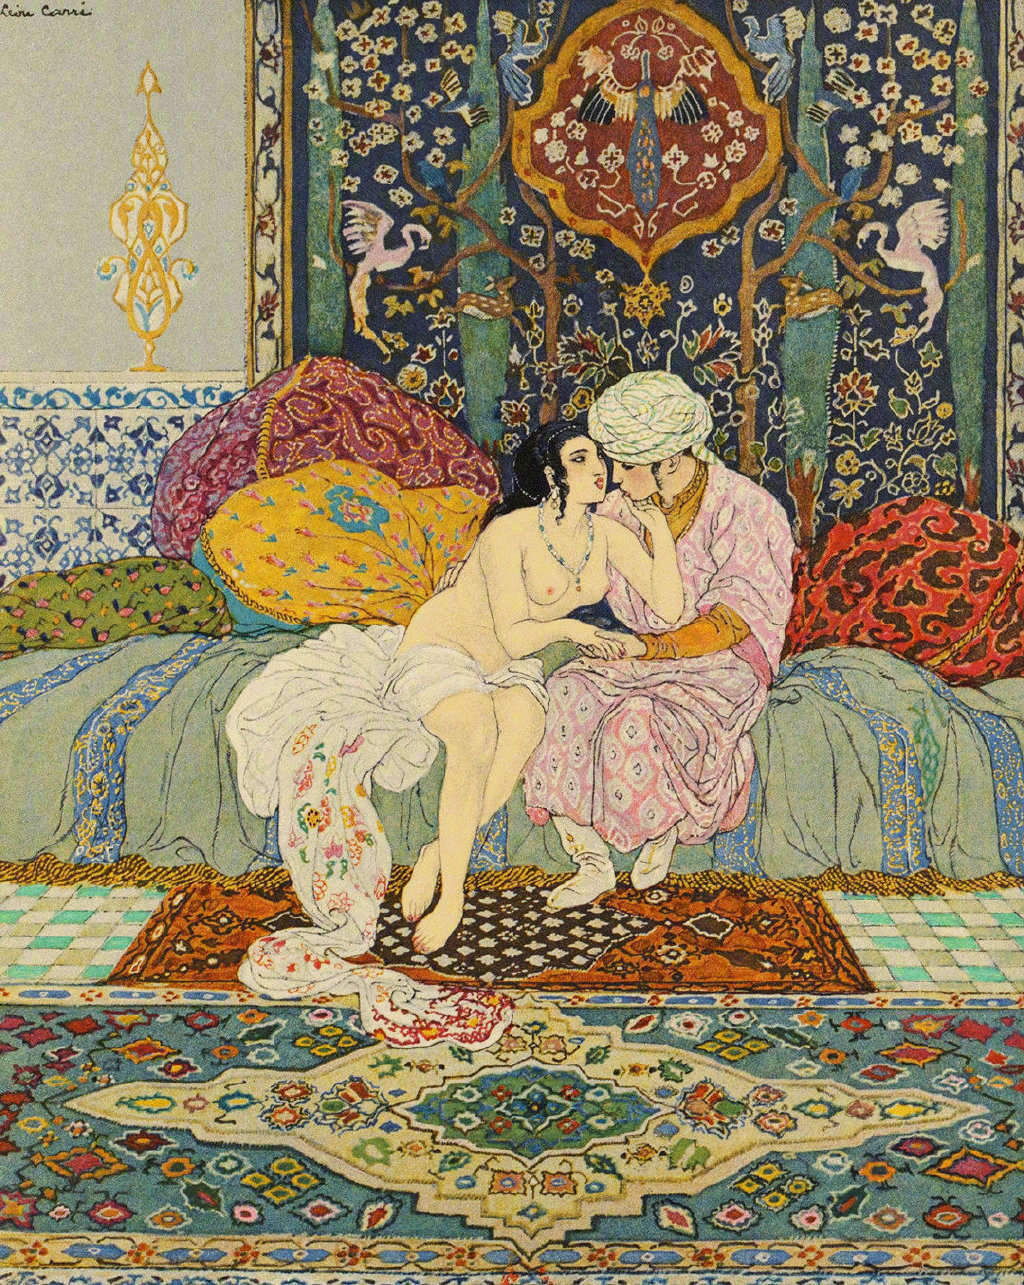
\includegraphics[height=\figsize]{illustrations/volume_1/T01, n0032(3) - Histoire de Douce-Amie.jpg}
\end{figure}

\textit{\\
"...Ali-Nour, ivre, s’avança, se jeta sur le divan, aux côtés de Douce-Amie. Et le couple s’enlaça."} \\
—T01, n0032(3) - Histoire de Douce-Amie \\~\\
\textit{"Al\={\i}-N\=ur threw himself on the couch by Sweet-Friend's side, drunken for very joy, and they gripped each other."} \\
—V01, n0032(3) - The tale of Sweet-Friend

\newpage

\section{n0034}
\textbf{\Large{The tale of Sweet-Friend}} \\

\begin{figure}[ht]
\centering
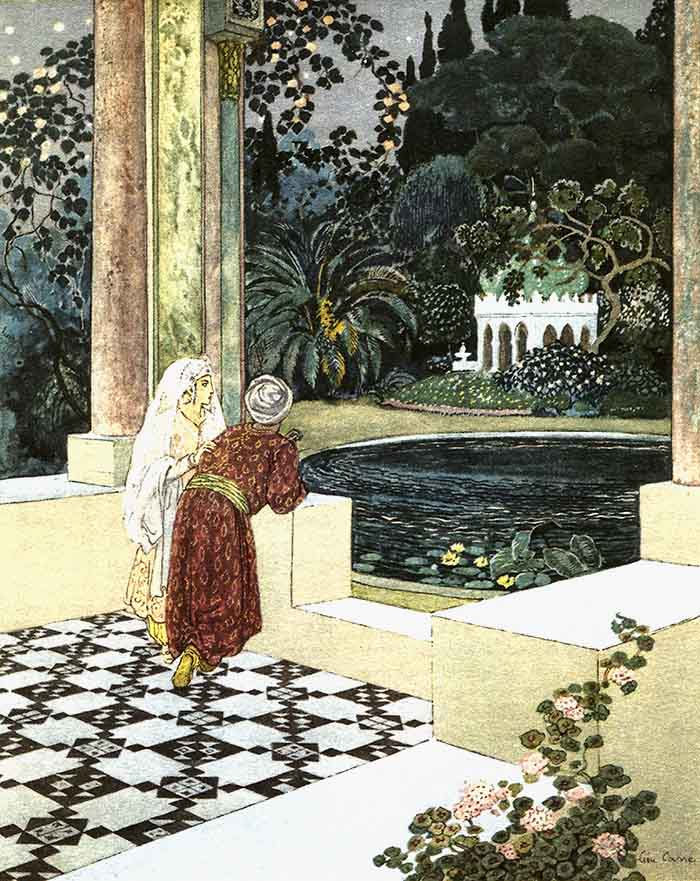
\includegraphics[height=\figsize]{illustrations/volume_1/T01, n0034 - Histoire de Douce-Amie.jpg}
\end{figure}

\textit{\\
"...ils mangèrent leur plein ; puis ils se lavèrent les mains, et de nouveau allèrent s’accouder à la fenêtre et regarder les arbres chargés de leurs beaux fruits."} \\
—T01, n0034 - Histoire de Douce-Amie \\~\\
\textit{"…they feasted abundantly. Then, after washing their hands, they returned to the window and stood looking out."} \\
—V01, n0034 - The tale of Sweet-Friend

\newpage

\section{n0035}
\textbf{\Large{The tale of Sweet-Friend}} \\

\begin{figure}[ht]
\centering
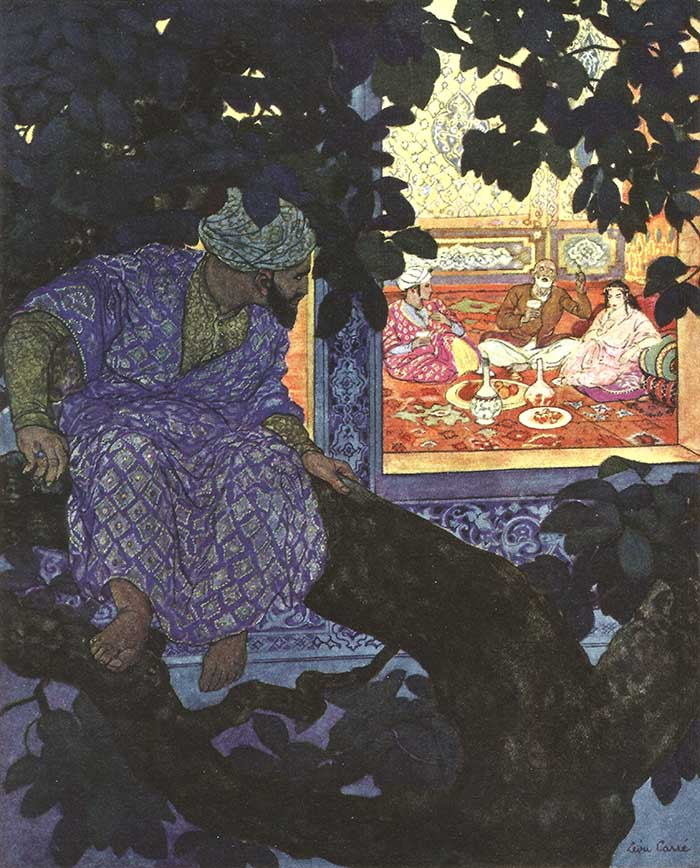
\includegraphics[height=\figsize]{illustrations/volume_1/T01, n0035 - Histoire de Douce-Amie.jpg}
\end{figure}

\textit{\\
"...le khalifat monta sur l’arbre, et ne cessa de grimper d’une branche à une autre branche qu’il n’eût atteint la branche qui était directement en face de l’une des fenêtres. Il s’assit alors sur la branche et regarda à travers la fenêtre."} \\
—T01, n0035 - Histoire de Douce-Amie \\~\\
\textit{"...the Khal\={\i}fah climbed, with Jafar s assistance, into a high nut tree and raised himself branch by branch until he could look through one of the windows."} \\
—V01, n0035 - The tale of Sweet-Friend

\newpage

\section{n0039}
\textbf{\Large{The tale of Gh\=anim Ibn Ayy\=ub [The tale of the negro Bakhait]}} \\

\begin{figure}[ht]
\centering
\includegraphics[height=\figsize]{illustrations/volume_1/T01, n0039 - Histoire de Ghanem Ben-Ayoub [Histoire du nègre Bakhita].jpg}
\end{figure}

\textit{\\
"Ghanem prit alors un caillou et se mit à frapper sur le cadenas qui fermait le couvercle de la caisse et finit par le casser. Et il leva le couvercle, et il trouva dans la caisse une adolescente, non point morte, mais endormie, car sa respiration montait et descendait d’une façon douce et réglée, et elle devait être seulement sous l’effet du banj."} \\
—T01, n0039 - Histoire de Ghanem Ben-Ayoub [Histoire du nègre Bakhita] \\~\\
\textit{"...picking up a stone, he broke the locks and threw back the lid. Inside was a sleeping girl, drugged seemingly with banj, whose bosom rose and fell in regular breathing."} \\
—V01, n0039 - The tale of Gh\=anim Ibn Ayy\=ub [The tale of the negro Bakhait]

\newpage

\section{n0041}
\textbf{\Large{The tale of Gh\=anim Ibn Ayy\=ub}} \\

\begin{figure}[ht]
\centering
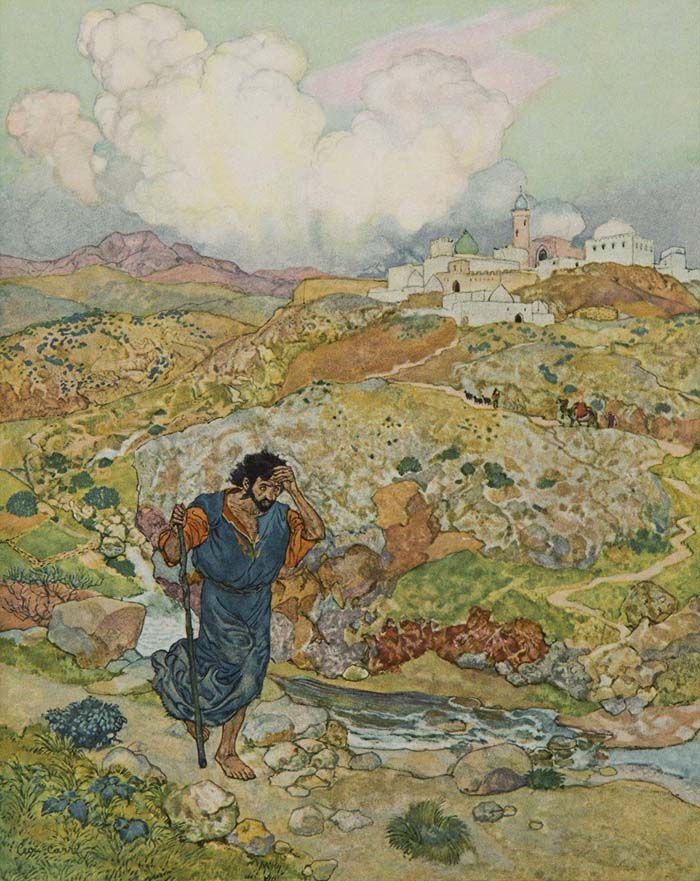
\includegraphics[height=\figsize]{illustrations/volume_1/T01, n0041 - Histoire de Ghanem Ben-Ayoub.jpg}
\end{figure}

\textit{\\
"...une fois sorti de Baghdad, il se mit à marcher et à pleurer jusqu’à ce que son cœur se fût émietté ; et il continua de la sorte, sans manger et sans boire, jusqu’à la fin de la journée ; et la faim et la douleur l’avaient affaibli."} \\
—T01, n0041 - Histoire de Ghanem Ben-Ayoub \\~\\
\textit{"He walked away from Baghd\=ad, weeping as if his heart were broken, and journeyed all day without eating or drinking…"} \\
—V01, n0041 - The tale of Gh\=anim Ibn Ayy\=ub

\end{document}